\documentclass[twoside]{book}

% Packages required by doxygen
\usepackage{calc}
\usepackage{doxygen}
\usepackage{graphicx}
\usepackage[utf8]{inputenc}
\usepackage{makeidx}
\usepackage{multicol}
\usepackage{multirow}
\usepackage{textcomp}
\usepackage[table]{xcolor}

% Font selection
\usepackage[T1]{fontenc}
\usepackage{mathptmx}
\usepackage[scaled=.90]{helvet}
\usepackage{courier}
\usepackage{amssymb}
\usepackage{sectsty}
\renewcommand{\familydefault}{\sfdefault}
\allsectionsfont{%
  \fontseries{bc}\selectfont%
  \color{darkgray}%
}
\renewcommand{\DoxyLabelFont}{%
  \fontseries{bc}\selectfont%
  \color{darkgray}%
}

% Page & text layout
\usepackage{geometry}
\geometry{%
  a4paper,%
  top=2.5cm,%
  bottom=2.5cm,%
  left=2.5cm,%
  right=2.5cm%
}
\tolerance=750
\hfuzz=15pt
\hbadness=750
\setlength{\emergencystretch}{15pt}
\setlength{\parindent}{0cm}
\setlength{\parskip}{0.2cm}
\makeatletter
\renewcommand{\paragraph}{%
  \@startsection{paragraph}{4}{0ex}{-1.0ex}{1.0ex}{%
    \normalfont\normalsize\bfseries\SS@parafont%
  }%
}
\renewcommand{\subparagraph}{%
  \@startsection{subparagraph}{5}{0ex}{-1.0ex}{1.0ex}{%
    \normalfont\normalsize\bfseries\SS@subparafont%
  }%
}
\makeatother

% Headers & footers
\usepackage{fancyhdr}
\pagestyle{fancyplain}
\fancyhead[LE]{\fancyplain{}{\bfseries\thepage}}
\fancyhead[CE]{\fancyplain{}{}}
\fancyhead[RE]{\fancyplain{}{\bfseries\leftmark}}
\fancyhead[LO]{\fancyplain{}{\bfseries\rightmark}}
\fancyhead[CO]{\fancyplain{}{}}
\fancyhead[RO]{\fancyplain{}{\bfseries\thepage}}
\fancyfoot[LE]{\fancyplain{}{}}
\fancyfoot[CE]{\fancyplain{}{}}
\fancyfoot[RE]{\fancyplain{}{\bfseries\scriptsize Generated on Mon Mar 20 2017 19\-:56\-:17 for My Project by Doxygen }}
\fancyfoot[LO]{\fancyplain{}{\bfseries\scriptsize Generated on Mon Mar 20 2017 19\-:56\-:17 for My Project by Doxygen }}
\fancyfoot[CO]{\fancyplain{}{}}
\fancyfoot[RO]{\fancyplain{}{}}
\renewcommand{\footrulewidth}{0.4pt}
\renewcommand{\chaptermark}[1]{%
  \markboth{#1}{}%
}
\renewcommand{\sectionmark}[1]{%
  \markright{\thesection\ #1}%
}

% Indices & bibliography
\usepackage{natbib}
\usepackage[titles]{tocloft}
\setcounter{tocdepth}{3}
\setcounter{secnumdepth}{5}
\makeindex

% Hyperlinks (required, but should be loaded last)
\usepackage{ifpdf}
\ifpdf
  \usepackage[pdftex,pagebackref=true]{hyperref}
\else
  \usepackage[ps2pdf,pagebackref=true]{hyperref}
\fi
\hypersetup{%
  colorlinks=true,%
  linkcolor=blue,%
  citecolor=blue,%
  unicode%
}

% Custom commands
\newcommand{\clearemptydoublepage}{%
  \newpage{\pagestyle{empty}\cleardoublepage}%
}


%===== C O N T E N T S =====

\begin{document}

% Titlepage & ToC
\hypersetup{pageanchor=false}
\pagenumbering{roman}
\begin{titlepage}
\vspace*{7cm}
\begin{center}%
{\Large My Project }\\
\vspace*{1cm}
{\large Generated by Doxygen 1.8.6}\\
\vspace*{0.5cm}
{\small Mon Mar 20 2017 19:56:17}\\
\end{center}
\end{titlepage}
\clearemptydoublepage
\tableofcontents
\clearemptydoublepage
\pagenumbering{arabic}
\hypersetup{pageanchor=true}

%--- Begin generated contents ---
\chapter{Guten\-\_\-\-Tag}
\label{md_README}
\hypertarget{md_README}{}
Project for a H\-C\-I class at Université de Nantes. The main purpose of this project is to create an application to tag files and repositories.
\begin{DoxyItemize}
\item using Qt A\-P\-I
\end{DoxyItemize}

Authors \-: Jonathan Bonnaud \& Kevin Espasa 
\chapter{Hierarchical Index}
\section{Class Hierarchy}
This inheritance list is sorted roughly, but not completely, alphabetically\-:\begin{DoxyCompactList}
\item Q\-Dialog\begin{DoxyCompactList}
\item \contentsline{section}{addtagdialog}{\pageref{classaddtagdialog}}{}
\item \contentsline{section}{deltagdialog}{\pageref{classdeltagdialog}}{}
\end{DoxyCompactList}
\item Q\-Main\-Window\begin{DoxyCompactList}
\item \contentsline{section}{Main\-Window}{\pageref{classMainWindow}}{}
\end{DoxyCompactList}
\item Q\-Widget\begin{DoxyCompactList}
\item \contentsline{section}{explorerlayout}{\pageref{classexplorerlayout}}{}
\item \contentsline{section}{taglayout}{\pageref{classtaglayout}}{}
\item \contentsline{section}{xmldom}{\pageref{classxmldom}}{}
\end{DoxyCompactList}
\item \contentsline{section}{tag}{\pageref{classtag}}{}
\end{DoxyCompactList}

\chapter{Class Index}
\section{Class List}
Here are the classes, structs, unions and interfaces with brief descriptions\-:\begin{DoxyCompactList}
\item\contentsline{section}{\hyperlink{classaddtagdialog}{addtagdialog} }{\pageref{classaddtagdialog}}{}
\item\contentsline{section}{\hyperlink{classdeltagdialog}{deltagdialog} }{\pageref{classdeltagdialog}}{}
\item\contentsline{section}{\hyperlink{classexplorerlayout}{explorerlayout} }{\pageref{classexplorerlayout}}{}
\item\contentsline{section}{\hyperlink{classMainWindow}{Main\-Window} }{\pageref{classMainWindow}}{}
\item\contentsline{section}{\hyperlink{classtag}{tag} }{\pageref{classtag}}{}
\item\contentsline{section}{\hyperlink{classtaglayout}{taglayout} }{\pageref{classtaglayout}}{}
\item\contentsline{section}{\hyperlink{classxmldom}{xmldom} }{\pageref{classxmldom}}{}
\end{DoxyCompactList}

\chapter{File Index}
\section{File List}
Here is a list of all documented files with brief descriptions\-:\begin{DoxyCompactList}
\item\contentsline{section}{\hyperlink{addtagdialog_8hpp}{addtagdialog.\-hpp} \\*Classe permettant l'affichage de la boite de dialog d'ajout d'un tag }{\pageref{addtagdialog_8hpp}}{}
\item\contentsline{section}{\hyperlink{deltagdialog_8hpp}{deltagdialog.\-hpp} \\*Classe permettant l'affichage de la boite de dialog de suppression d'un ou plusieurs tags }{\pageref{deltagdialog_8hpp}}{}
\item\contentsline{section}{\hyperlink{explorerlayout_8hpp}{explorerlayout.\-hpp} \\*Widget affichant les fichiers et les informations qui sont associées }{\pageref{explorerlayout_8hpp}}{}
\item\contentsline{section}{{\bfseries mainwindow.\-h} }{\pageref{mainwindow_8h}}{}
\item\contentsline{section}{\hyperlink{tag_8hpp}{tag.\-hpp} \\*Classe definissant un tag }{\pageref{tag_8hpp}}{}
\item\contentsline{section}{\hyperlink{taglayout_8hpp}{taglayout.\-hpp} \\*Classe definissant les tags }{\pageref{taglayout_8hpp}}{}
\item\contentsline{section}{\hyperlink{xmldom_8hpp}{xmldom.\-hpp} \\*Classe permettant la lecture et l'ecrire d'un xml }{\pageref{xmldom_8hpp}}{}
\end{DoxyCompactList}

\chapter{Class Documentation}
\hypertarget{classaddtagdialog}{\section{addtagdialog Class Reference}
\label{classaddtagdialog}\index{addtagdialog@{addtagdialog}}
}
Inheritance diagram for addtagdialog\-:\begin{figure}[H]
\begin{center}
\leavevmode
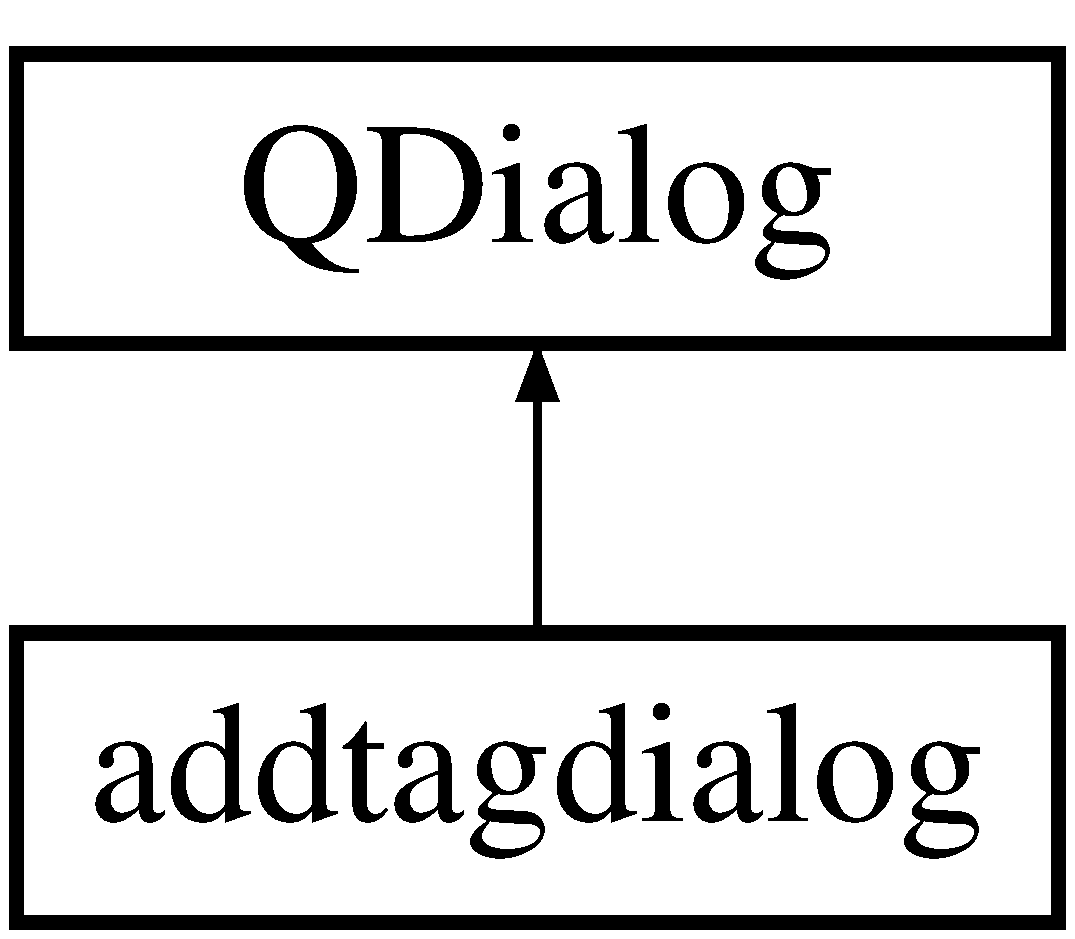
\includegraphics[height=2.000000cm]{classaddtagdialog}
\end{center}
\end{figure}
\subsection*{Public Slots}
\begin{DoxyCompactItemize}
\item 
\hypertarget{classaddtagdialog_afaf3ddf489176280fe73325d128d500c}{void \hyperlink{classaddtagdialog_afaf3ddf489176280fe73325d128d500c}{accept\-\_\-add\-\_\-tag} ()}\label{classaddtagdialog_afaf3ddf489176280fe73325d128d500c}

\begin{DoxyCompactList}\small\item\em slot associé au boutton valider testant si un bouton peut être créé \end{DoxyCompactList}\end{DoxyCompactItemize}
\subsection*{Signals}
\begin{DoxyCompactItemize}
\item 
\hypertarget{classaddtagdialog_aef3fda151058d8a0600873ca2f557d92}{void {\bfseries tag\-\_\-added} ()}\label{classaddtagdialog_aef3fda151058d8a0600873ca2f557d92}

\end{DoxyCompactItemize}
\subsection*{Public Member Functions}
\begin{DoxyCompactItemize}
\item 
\hyperlink{classaddtagdialog_a74206d3637d63e21311304a17e593787}{addtagdialog} (Q\-Vector$<$ \hyperlink{classtag}{tag} $\ast$ $>$ $\ast$taglist)
\begin{DoxyCompactList}\small\item\em constructeur de la classe \end{DoxyCompactList}\item 
\hypertarget{classaddtagdialog_a1a448e66aee6c358a35b7c1fa9a98579}{void \hyperlink{classaddtagdialog_a1a448e66aee6c358a35b7c1fa9a98579}{add\-\_\-tag\-\_\-to\-\_\-list} ()}\label{classaddtagdialog_a1a448e66aee6c358a35b7c1fa9a98579}

\begin{DoxyCompactList}\small\item\em procédure créant un boutton \end{DoxyCompactList}\end{DoxyCompactItemize}


\subsection{Constructor \& Destructor Documentation}
\hypertarget{classaddtagdialog_a74206d3637d63e21311304a17e593787}{\index{addtagdialog@{addtagdialog}!addtagdialog@{addtagdialog}}
\index{addtagdialog@{addtagdialog}!addtagdialog@{addtagdialog}}
\subsubsection[{addtagdialog}]{\setlength{\rightskip}{0pt plus 5cm}addtagdialog\-::addtagdialog (
\begin{DoxyParamCaption}
\item[{Q\-Vector$<$ {\bf tag} $\ast$ $>$ $\ast$}]{taglist}
\end{DoxyParamCaption}
)}}\label{classaddtagdialog_a74206d3637d63e21311304a17e593787}


constructeur de la classe 


\begin{DoxyParams}{Parameters}
{\em taglist} & adresse du taglist \\
\hline
\end{DoxyParams}


The documentation for this class was generated from the following files\-:\begin{DoxyCompactItemize}
\item 
\hyperlink{addtagdialog_8hpp}{addtagdialog.\-hpp}\item 
addtagdialog.\-cpp\end{DoxyCompactItemize}

\hypertarget{classdeltagdialog}{\section{deltagdialog Class Reference}
\label{classdeltagdialog}\index{deltagdialog@{deltagdialog}}
}
Inheritance diagram for deltagdialog\-:\begin{figure}[H]
\begin{center}
\leavevmode
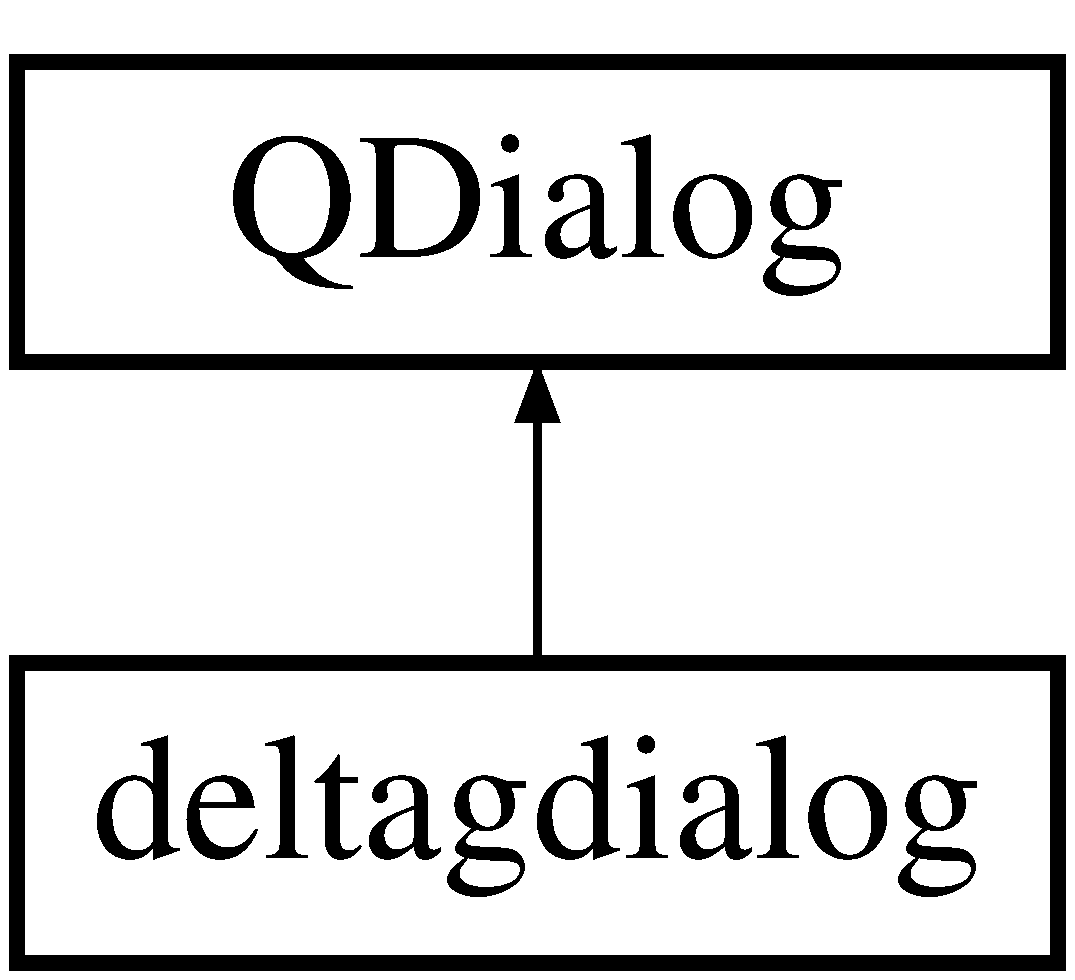
\includegraphics[height=2.000000cm]{classdeltagdialog}
\end{center}
\end{figure}
\subsection*{Public Slots}
\begin{DoxyCompactItemize}
\item 
\hypertarget{classdeltagdialog_ab221c23d6e90da92e9944ac3a885c504}{void \hyperlink{classdeltagdialog_ab221c23d6e90da92e9944ac3a885c504}{print\-\_\-list\-\_\-checkbox} ()}\label{classdeltagdialog_ab221c23d6e90da92e9944ac3a885c504}

\begin{DoxyCompactList}\small\item\em affiche la liste de checkbox \end{DoxyCompactList}\item 
\hypertarget{classdeltagdialog_a43da5e859752a49256dce0337ff1b9d1}{void \hyperlink{classdeltagdialog_a43da5e859752a49256dce0337ff1b9d1}{accept\-\_\-del\-\_\-tag} ()}\label{classdeltagdialog_a43da5e859752a49256dce0337ff1b9d1}

\begin{DoxyCompactList}\small\item\em slot supprimant les tags. \end{DoxyCompactList}\end{DoxyCompactItemize}
\subsection*{Signals}
\begin{DoxyCompactItemize}
\item 
\hypertarget{classdeltagdialog_aec21287cbed72964487a26ecd9d56264}{void {\bfseries tag\-\_\-deleted} ()}\label{classdeltagdialog_aec21287cbed72964487a26ecd9d56264}

\end{DoxyCompactItemize}
\subsection*{Public Member Functions}
\begin{DoxyCompactItemize}
\item 
\hyperlink{classdeltagdialog_a7ed02b8021e05676d41180d03f3af36d}{deltagdialog} (Q\-Vector$<$ \hyperlink{classtag}{tag} $\ast$ $>$ $\ast$taglist)
\begin{DoxyCompactList}\small\item\em constructeur de la classe \end{DoxyCompactList}\item 
\hypertarget{classdeltagdialog_a0f25892d880bfaea6ea11d2ca5fed54c}{void \hyperlink{classdeltagdialog_a0f25892d880bfaea6ea11d2ca5fed54c}{del\-\_\-tag\-\_\-from\-\_\-list} ()}\label{classdeltagdialog_a0f25892d880bfaea6ea11d2ca5fed54c}

\begin{DoxyCompactList}\small\item\em supprime un tag de la list \end{DoxyCompactList}\item 
Q\-List$<$ int $>$ $\ast$ \hyperlink{classdeltagdialog_a27c650a71c6874049236e71b2e261b01}{get\-Tab} ()
\begin{DoxyCompactList}\small\item\em retourne la liste d'indexe des tags supprimés \end{DoxyCompactList}\end{DoxyCompactItemize}


\subsection{Constructor \& Destructor Documentation}
\hypertarget{classdeltagdialog_a7ed02b8021e05676d41180d03f3af36d}{\index{deltagdialog@{deltagdialog}!deltagdialog@{deltagdialog}}
\index{deltagdialog@{deltagdialog}!deltagdialog@{deltagdialog}}
\subsubsection[{deltagdialog}]{\setlength{\rightskip}{0pt plus 5cm}deltagdialog\-::deltagdialog (
\begin{DoxyParamCaption}
\item[{Q\-Vector$<$ {\bf tag} $\ast$ $>$ $\ast$}]{taglist}
\end{DoxyParamCaption}
)}}\label{classdeltagdialog_a7ed02b8021e05676d41180d03f3af36d}


constructeur de la classe 


\begin{DoxyParams}{Parameters}
{\em taglist} & adresse du taglist \\
\hline
\end{DoxyParams}


\subsection{Member Function Documentation}
\hypertarget{classdeltagdialog_a27c650a71c6874049236e71b2e261b01}{\index{deltagdialog@{deltagdialog}!get\-Tab@{get\-Tab}}
\index{get\-Tab@{get\-Tab}!deltagdialog@{deltagdialog}}
\subsubsection[{get\-Tab}]{\setlength{\rightskip}{0pt plus 5cm}Q\-List$<$ int $>$ $\ast$ deltagdialog\-::get\-Tab (
\begin{DoxyParamCaption}
{}
\end{DoxyParamCaption}
)}}\label{classdeltagdialog_a27c650a71c6874049236e71b2e261b01}


retourne la liste d'indexe des tags supprimés 

\begin{DoxyReturn}{Returns}
Q\-List 
\end{DoxyReturn}


The documentation for this class was generated from the following files\-:\begin{DoxyCompactItemize}
\item 
\hyperlink{deltagdialog_8hpp}{deltagdialog.\-hpp}\item 
deltagdialog.\-cpp\end{DoxyCompactItemize}

\hypertarget{classexplorerlayout}{\section{explorerlayout Class Reference}
\label{classexplorerlayout}\index{explorerlayout@{explorerlayout}}
}
Inheritance diagram for explorerlayout\-:\begin{figure}[H]
\begin{center}
\leavevmode
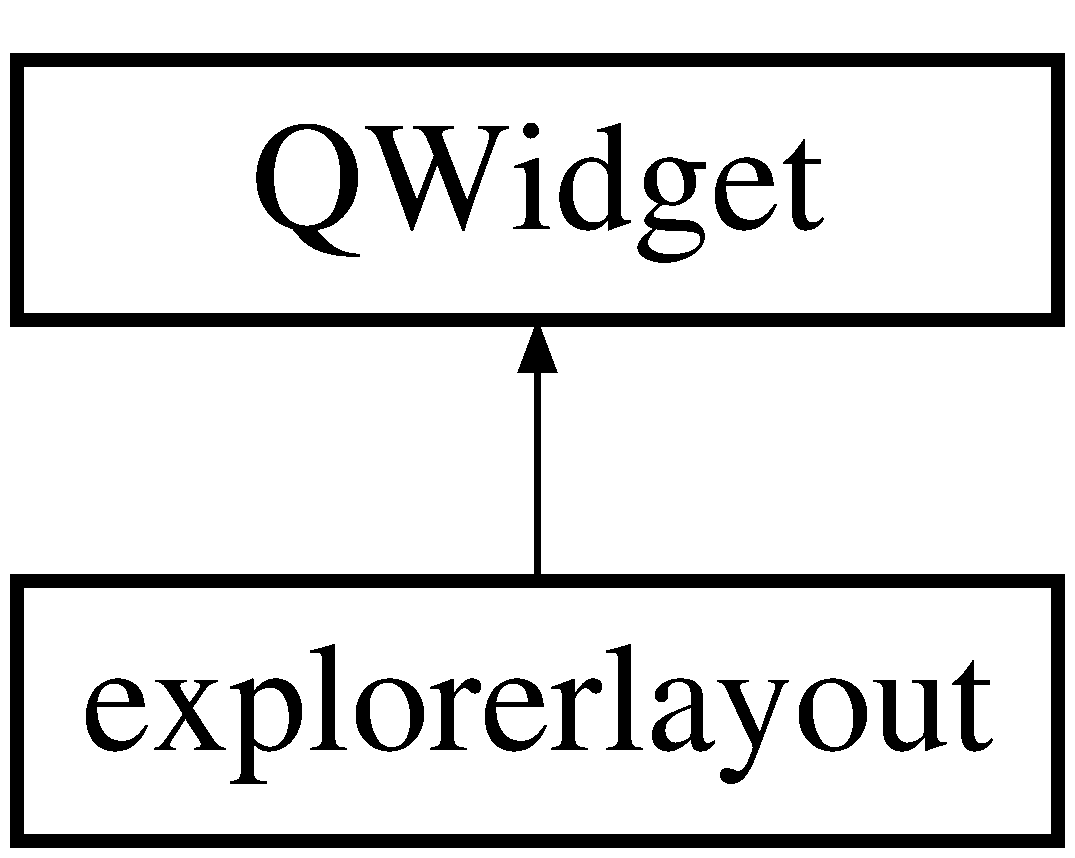
\includegraphics[height=2.000000cm]{classexplorerlayout}
\end{center}
\end{figure}
\subsection*{Public Slots}
\begin{DoxyCompactItemize}
\item 
void \hyperlink{classexplorerlayout_a901d318100af1524b51b0075d9626c01}{on\-\_\-qtableview\-\_\-double\-Clicked} (const Q\-Model\-Index \&index)
\begin{DoxyCompactList}\small\item\em slot permettant lors d'un double clic de rentrer dans le dossier. \end{DoxyCompactList}\item 
\hypertarget{classexplorerlayout_aa96e3819021c89ea58df68a34e599b22}{void \hyperlink{classexplorerlayout_aa96e3819021c89ea58df68a34e599b22}{on\-\_\-path\-\_\-return\-Pressed} ()}\label{classexplorerlayout_aa96e3819021c89ea58df68a34e599b22}

\begin{DoxyCompactList}\small\item\em slot associé a l'edit text lorsque l'on appuie sur entrée, on va au path donné s'il existe. \end{DoxyCompactList}\item 
\hypertarget{classexplorerlayout_ade8d3fbd3d0e61cb409191736ab844e6}{void \hyperlink{classexplorerlayout_ade8d3fbd3d0e61cb409191736ab844e6}{on\-\_\-backbutton\-\_\-clicked} ()}\label{classexplorerlayout_ade8d3fbd3d0e61cb409191736ab844e6}

\begin{DoxyCompactList}\small\item\em slot associé au boutton \char`\"{}$<$\char`\"{} permettant le retour en arriere pour le path. \end{DoxyCompactList}\item 
void \hyperlink{classexplorerlayout_afb5f67a2903743d8a8374f5160ff5d25}{on\-\_\-qtableview\-\_\-clicked} (const Q\-Model\-Index \&index)
\begin{DoxyCompactList}\small\item\em slot associé à la table view affichant dans la table la liste des tags associés au fichier sélectionné dans le table view \end{DoxyCompactList}\item 
\hypertarget{classexplorerlayout_a08d4b2c695d42645f4d29f96e90ed07f}{void {\bfseries hide\-List\-Files} (int index)}\label{classexplorerlayout_a08d4b2c695d42645f4d29f96e90ed07f}

\end{DoxyCompactItemize}
\subsection*{Public Member Functions}
\begin{DoxyCompactItemize}
\item 
\hyperlink{classexplorerlayout_aed9ef211abfc6af064bda787445981e1}{explorerlayout} (\hyperlink{classxmldom}{xmldom} $\ast$xdom)
\begin{DoxyCompactList}\small\item\em constructeur du widget. \end{DoxyCompactList}\item 
Q\-Table\-View $\ast$ \hyperlink{classexplorerlayout_aaa3d4b0374eebf3bc851080447ff9e28}{get\-Table\-View} ()
\begin{DoxyCompactList}\small\item\em fonction retournant la table view. \end{DoxyCompactList}\item 
Q\-Model\-Index\-List \hyperlink{classexplorerlayout_a4132f3f08f7d8d25e7e818ab68f5c566}{get\-Index\-Table\-View} ()
\begin{DoxyCompactList}\small\item\em fonction retournant le pointeur du tableau des indexes sélectionnés. \end{DoxyCompactList}\item 
Q\-String \hyperlink{classexplorerlayout_a4c2cdee19ac9098602d404eae2d5bcf2}{get\-Path} ()
\begin{DoxyCompactList}\small\item\em fonction retournant le path de la editline. \end{DoxyCompactList}\item 
void \hyperlink{classexplorerlayout_a2046b6c80a021c39ce6630d55be09c98}{filter} (Q\-Push\-Button $\ast$button)
\begin{DoxyCompactList}\small\item\em procédure de filtre, elle affiche à la place de la table view la liste des fichiers associés à un tag donné. \end{DoxyCompactList}\end{DoxyCompactItemize}


\subsection{Constructor \& Destructor Documentation}
\hypertarget{classexplorerlayout_aed9ef211abfc6af064bda787445981e1}{\index{explorerlayout@{explorerlayout}!explorerlayout@{explorerlayout}}
\index{explorerlayout@{explorerlayout}!explorerlayout@{explorerlayout}}
\subsubsection[{explorerlayout}]{\setlength{\rightskip}{0pt plus 5cm}explorerlayout\-::explorerlayout (
\begin{DoxyParamCaption}
\item[{{\bf xmldom} $\ast$}]{xdom}
\end{DoxyParamCaption}
)}}\label{classexplorerlayout_aed9ef211abfc6af064bda787445981e1}


constructeur du widget. 


\begin{DoxyParams}{Parameters}
{\em xdom} & le xml comportant les informations sur les tags. \\
\hline
\end{DoxyParams}


\subsection{Member Function Documentation}
\hypertarget{classexplorerlayout_a2046b6c80a021c39ce6630d55be09c98}{\index{explorerlayout@{explorerlayout}!filter@{filter}}
\index{filter@{filter}!explorerlayout@{explorerlayout}}
\subsubsection[{filter}]{\setlength{\rightskip}{0pt plus 5cm}void explorerlayout\-::filter (
\begin{DoxyParamCaption}
\item[{Q\-Push\-Button $\ast$}]{button}
\end{DoxyParamCaption}
)}}\label{classexplorerlayout_a2046b6c80a021c39ce6630d55be09c98}


procédure de filtre, elle affiche à la place de la table view la liste des fichiers associés à un tag donné. 


\begin{DoxyParams}{Parameters}
{\em name,le} & nom du boutton. \\
\hline
\end{DoxyParams}
\hypertarget{classexplorerlayout_a4132f3f08f7d8d25e7e818ab68f5c566}{\index{explorerlayout@{explorerlayout}!get\-Index\-Table\-View@{get\-Index\-Table\-View}}
\index{get\-Index\-Table\-View@{get\-Index\-Table\-View}!explorerlayout@{explorerlayout}}
\subsubsection[{get\-Index\-Table\-View}]{\setlength{\rightskip}{0pt plus 5cm}Q\-Model\-Index\-List explorerlayout\-::get\-Index\-Table\-View (
\begin{DoxyParamCaption}
{}
\end{DoxyParamCaption}
)}}\label{classexplorerlayout_a4132f3f08f7d8d25e7e818ab68f5c566}


fonction retournant le pointeur du tableau des indexes sélectionnés. 

\begin{DoxyReturn}{Returns}
Q\-Table\-View. 
\end{DoxyReturn}
\hypertarget{classexplorerlayout_a4c2cdee19ac9098602d404eae2d5bcf2}{\index{explorerlayout@{explorerlayout}!get\-Path@{get\-Path}}
\index{get\-Path@{get\-Path}!explorerlayout@{explorerlayout}}
\subsubsection[{get\-Path}]{\setlength{\rightskip}{0pt plus 5cm}Q\-String explorerlayout\-::get\-Path (
\begin{DoxyParamCaption}
{}
\end{DoxyParamCaption}
)}}\label{classexplorerlayout_a4c2cdee19ac9098602d404eae2d5bcf2}


fonction retournant le path de la editline. 

\begin{DoxyReturn}{Returns}
Q\-String. 
\end{DoxyReturn}
\hypertarget{classexplorerlayout_aaa3d4b0374eebf3bc851080447ff9e28}{\index{explorerlayout@{explorerlayout}!get\-Table\-View@{get\-Table\-View}}
\index{get\-Table\-View@{get\-Table\-View}!explorerlayout@{explorerlayout}}
\subsubsection[{get\-Table\-View}]{\setlength{\rightskip}{0pt plus 5cm}Q\-Table\-View $\ast$ explorerlayout\-::get\-Table\-View (
\begin{DoxyParamCaption}
{}
\end{DoxyParamCaption}
)}}\label{classexplorerlayout_aaa3d4b0374eebf3bc851080447ff9e28}


fonction retournant la table view. 

\begin{DoxyReturn}{Returns}
la table view. 
\end{DoxyReturn}
\hypertarget{classexplorerlayout_afb5f67a2903743d8a8374f5160ff5d25}{\index{explorerlayout@{explorerlayout}!on\-\_\-qtableview\-\_\-clicked@{on\-\_\-qtableview\-\_\-clicked}}
\index{on\-\_\-qtableview\-\_\-clicked@{on\-\_\-qtableview\-\_\-clicked}!explorerlayout@{explorerlayout}}
\subsubsection[{on\-\_\-qtableview\-\_\-clicked}]{\setlength{\rightskip}{0pt plus 5cm}void explorerlayout\-::on\-\_\-qtableview\-\_\-clicked (
\begin{DoxyParamCaption}
\item[{const Q\-Model\-Index \&}]{index}
\end{DoxyParamCaption}
)\hspace{0.3cm}{\ttfamily [slot]}}}\label{classexplorerlayout_afb5f67a2903743d8a8374f5160ff5d25}


slot associé à la table view affichant dans la table la liste des tags associés au fichier sélectionné dans le table view 


\begin{DoxyParams}{Parameters}
{\em index} & \\
\hline
\end{DoxyParams}
\hypertarget{classexplorerlayout_a901d318100af1524b51b0075d9626c01}{\index{explorerlayout@{explorerlayout}!on\-\_\-qtableview\-\_\-double\-Clicked@{on\-\_\-qtableview\-\_\-double\-Clicked}}
\index{on\-\_\-qtableview\-\_\-double\-Clicked@{on\-\_\-qtableview\-\_\-double\-Clicked}!explorerlayout@{explorerlayout}}
\subsubsection[{on\-\_\-qtableview\-\_\-double\-Clicked}]{\setlength{\rightskip}{0pt plus 5cm}void explorerlayout\-::on\-\_\-qtableview\-\_\-double\-Clicked (
\begin{DoxyParamCaption}
\item[{const Q\-Model\-Index \&}]{index}
\end{DoxyParamCaption}
)\hspace{0.3cm}{\ttfamily [slot]}}}\label{classexplorerlayout_a901d318100af1524b51b0075d9626c01}


slot permettant lors d'un double clic de rentrer dans le dossier. 


\begin{DoxyParams}{Parameters}
{\em index} & \\
\hline
\end{DoxyParams}


The documentation for this class was generated from the following files\-:\begin{DoxyCompactItemize}
\item 
\hyperlink{explorerlayout_8hpp}{explorerlayout.\-hpp}\item 
explorerlayout.\-cpp\end{DoxyCompactItemize}

\hypertarget{classMainWindow}{\section{Main\-Window Class Reference}
\label{classMainWindow}\index{Main\-Window@{Main\-Window}}
}
Inheritance diagram for Main\-Window\-:\begin{figure}[H]
\begin{center}
\leavevmode
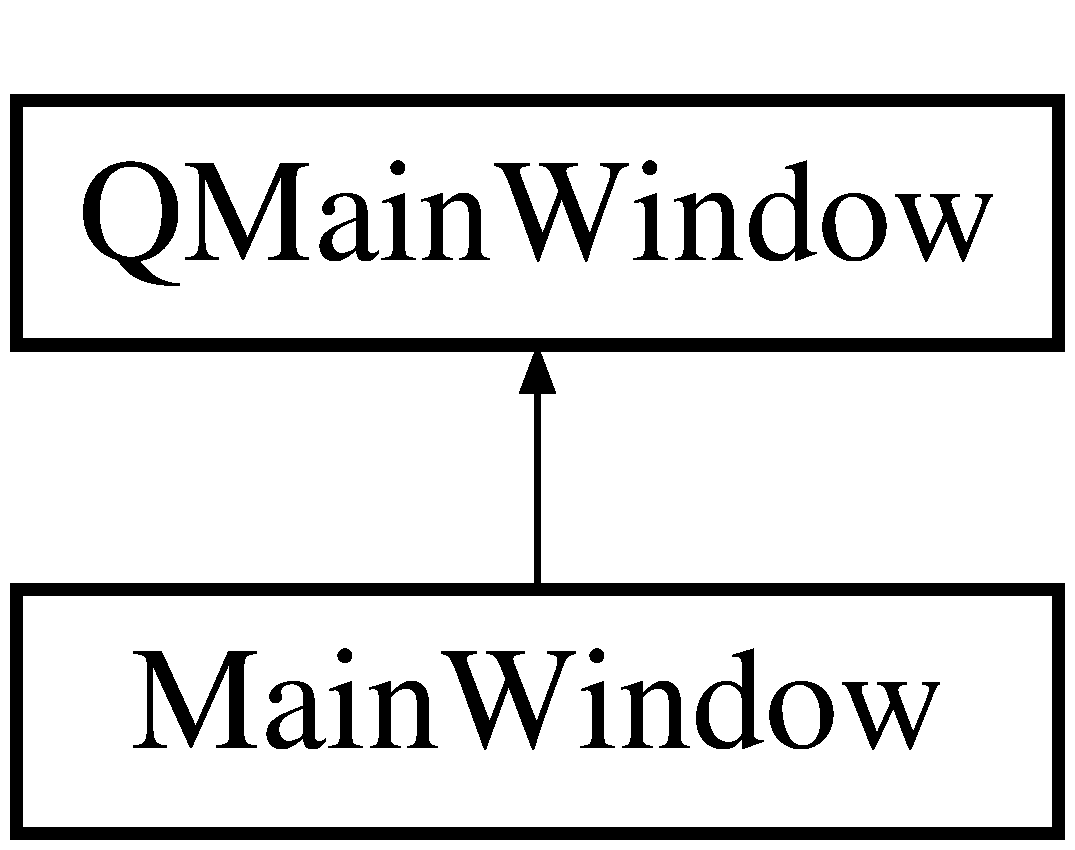
\includegraphics[height=2.000000cm]{classMainWindow}
\end{center}
\end{figure}
\subsection*{Public Slots}
\begin{DoxyCompactItemize}
\item 
\hypertarget{classMainWindow_a7be6a5d98970ac1a6296c6f9aee1e9bb}{void \hyperlink{classMainWindow_a7be6a5d98970ac1a6296c6f9aee1e9bb}{about} ()}\label{classMainWindow_a7be6a5d98970ac1a6296c6f9aee1e9bb}

\begin{DoxyCompactList}\small\item\em slot associé au boutton about \end{DoxyCompactList}\end{DoxyCompactItemize}
\subsection*{Public Member Functions}
\begin{DoxyCompactItemize}
\item 
\hypertarget{classMainWindow_a34c4b4207b46d11a4100c9b19f0e81bb}{\hyperlink{classMainWindow_a34c4b4207b46d11a4100c9b19f0e81bb}{Main\-Window} ()}\label{classMainWindow_a34c4b4207b46d11a4100c9b19f0e81bb}

\begin{DoxyCompactList}\small\item\em construteur de la classe \end{DoxyCompactList}\item 
\hypertarget{classMainWindow_ae98d00a93bc118200eeef9f9bba1dba7}{\hyperlink{classMainWindow_ae98d00a93bc118200eeef9f9bba1dba7}{$\sim$\-Main\-Window} ()}\label{classMainWindow_ae98d00a93bc118200eeef9f9bba1dba7}

\begin{DoxyCompactList}\small\item\em destructeur de la classe \end{DoxyCompactList}\end{DoxyCompactItemize}


The documentation for this class was generated from the following files\-:\begin{DoxyCompactItemize}
\item 
mainwindow.\-h\item 
mainwindow.\-cpp\end{DoxyCompactItemize}

\hypertarget{classtag}{\section{tag Class Reference}
\label{classtag}\index{tag@{tag}}
}
\subsection*{Public Member Functions}
\begin{DoxyCompactItemize}
\item 
\hypertarget{classtag_a2fa03e94e684be742a0f1a1a50fbafc9}{\hyperlink{classtag_a2fa03e94e684be742a0f1a1a50fbafc9}{tag} ()}\label{classtag_a2fa03e94e684be742a0f1a1a50fbafc9}

\begin{DoxyCompactList}\small\item\em constructeur par defaut d'un tag \end{DoxyCompactList}\item 
\hyperlink{classtag_aff22891fe1abf1ed5e9b5d440d0158d3}{tag} (Q\-String name, Q\-Color color)
\begin{DoxyCompactList}\small\item\em construteur du tag \end{DoxyCompactList}\item 
\hyperlink{classtag_a76b07b771d1600598aed98d118b94576}{tag} (Q\-String name, Q\-Color color, Q\-Vector$<$ Q\-String $>$ files)
\begin{DoxyCompactList}\small\item\em constructeur du tag \end{DoxyCompactList}\item 
Q\-Color \hyperlink{classtag_ab16256916b9d7bdbf0273ae48af8cc7d}{get\-Color} ()
\begin{DoxyCompactList}\small\item\em fonction retournant la couleur associé à un tag \end{DoxyCompactList}\item 
void \hyperlink{classtag_a90f4405518e74f1ccec80d198a735b77}{set\-Color} (Q\-Color color)
\begin{DoxyCompactList}\small\item\em modifie la couleur associé au tag \end{DoxyCompactList}\item 
Q\-String \hyperlink{classtag_a8cebe9849516a303817cb5a7a4ea9614}{get\-Name} ()
\begin{DoxyCompactList}\small\item\em fonction retournant le nom du tag \end{DoxyCompactList}\item 
void \hyperlink{classtag_a0566adcb0d18f06a37f456d9fb52ae9e}{set\-Name} (Q\-String name)
\begin{DoxyCompactList}\small\item\em modifie le nom associé au tag \end{DoxyCompactList}\item 
void \hyperlink{classtag_a0a0380b3ce237616186cd22e04c16005}{delete\-File} (Q\-String filename)
\begin{DoxyCompactList}\small\item\em procédure supprimant un fichier associé à un tag. \end{DoxyCompactList}\item 
void \hyperlink{classtag_a27bb06f6a7a0615db567df84d0357721}{add\-File} (Q\-String filename)
\begin{DoxyCompactList}\small\item\em procédure ajoutant un fichier à un tag \end{DoxyCompactList}\item 
void \hyperlink{classtag_aaadbc35ac88e71a9679188ce50d92ef9}{set\-Vector} (Q\-Vector$<$ Q\-String $>$ files)
\begin{DoxyCompactList}\small\item\em procédure modifiant le vecteur de fichier associé au tag \end{DoxyCompactList}\item 
Q\-Vector$<$ Q\-String $>$ \hyperlink{classtag_a444e286ff40c9aca8c7cc74032c764af}{get\-Vector} ()
\begin{DoxyCompactList}\small\item\em fonction retournant le vecteur de fichiers associé au tag \end{DoxyCompactList}\item 
bool \hyperlink{classtag_a59991e0c7cdf7cbaaf4e9b818a9d8084}{get\-Selected} ()
\begin{DoxyCompactList}\small\item\em fonction retournant le boolean si un tag est selectionne. \end{DoxyCompactList}\item 
void \hyperlink{classtag_a752cd9e4379c9cce40444a528310fc8c}{set\-Selected} (bool s)
\begin{DoxyCompactList}\small\item\em modifie si la valeur du boolean \end{DoxyCompactList}\end{DoxyCompactItemize}


\subsection{Constructor \& Destructor Documentation}
\hypertarget{classtag_aff22891fe1abf1ed5e9b5d440d0158d3}{\index{tag@{tag}!tag@{tag}}
\index{tag@{tag}!tag@{tag}}
\subsubsection[{tag}]{\setlength{\rightskip}{0pt plus 5cm}tag\-::tag (
\begin{DoxyParamCaption}
\item[{Q\-String}]{name, }
\item[{Q\-Color}]{color}
\end{DoxyParamCaption}
)}}\label{classtag_aff22891fe1abf1ed5e9b5d440d0158d3}


construteur du tag 


\begin{DoxyParams}{Parameters}
{\em name} & nom du tag \\
\hline
{\em color} & couleur qui lui est associée \\
\hline
\end{DoxyParams}
\hypertarget{classtag_a76b07b771d1600598aed98d118b94576}{\index{tag@{tag}!tag@{tag}}
\index{tag@{tag}!tag@{tag}}
\subsubsection[{tag}]{\setlength{\rightskip}{0pt plus 5cm}tag\-::tag (
\begin{DoxyParamCaption}
\item[{Q\-String}]{name, }
\item[{Q\-Color}]{color, }
\item[{Q\-Vector$<$ Q\-String $>$}]{files}
\end{DoxyParamCaption}
)}}\label{classtag_a76b07b771d1600598aed98d118b94576}


constructeur du tag 


\begin{DoxyParams}{Parameters}
{\em name} & nom du tag \\
\hline
{\em color} & couleur qui lui est associée \\
\hline
{\em files} & liste des fichiers qui sont taggé par le tag \\
\hline
\end{DoxyParams}


\subsection{Member Function Documentation}
\hypertarget{classtag_a27bb06f6a7a0615db567df84d0357721}{\index{tag@{tag}!add\-File@{add\-File}}
\index{add\-File@{add\-File}!tag@{tag}}
\subsubsection[{add\-File}]{\setlength{\rightskip}{0pt plus 5cm}void tag\-::add\-File (
\begin{DoxyParamCaption}
\item[{Q\-String}]{filename}
\end{DoxyParamCaption}
)}}\label{classtag_a27bb06f6a7a0615db567df84d0357721}


procédure ajoutant un fichier à un tag 


\begin{DoxyParams}{Parameters}
{\em filename} & le nom du fichier \\
\hline
\end{DoxyParams}
\hypertarget{classtag_a0a0380b3ce237616186cd22e04c16005}{\index{tag@{tag}!delete\-File@{delete\-File}}
\index{delete\-File@{delete\-File}!tag@{tag}}
\subsubsection[{delete\-File}]{\setlength{\rightskip}{0pt plus 5cm}void tag\-::delete\-File (
\begin{DoxyParamCaption}
\item[{Q\-String}]{filename}
\end{DoxyParamCaption}
)}}\label{classtag_a0a0380b3ce237616186cd22e04c16005}


procédure supprimant un fichier associé à un tag. 


\begin{DoxyParams}{Parameters}
{\em filename} & le nom du fichier \\
\hline
\end{DoxyParams}
\hypertarget{classtag_ab16256916b9d7bdbf0273ae48af8cc7d}{\index{tag@{tag}!get\-Color@{get\-Color}}
\index{get\-Color@{get\-Color}!tag@{tag}}
\subsubsection[{get\-Color}]{\setlength{\rightskip}{0pt plus 5cm}Q\-Color tag\-::get\-Color (
\begin{DoxyParamCaption}
{}
\end{DoxyParamCaption}
)}}\label{classtag_ab16256916b9d7bdbf0273ae48af8cc7d}


fonction retournant la couleur associé à un tag 

\begin{DoxyReturn}{Returns}
Q\-Color 
\end{DoxyReturn}
\hypertarget{classtag_a8cebe9849516a303817cb5a7a4ea9614}{\index{tag@{tag}!get\-Name@{get\-Name}}
\index{get\-Name@{get\-Name}!tag@{tag}}
\subsubsection[{get\-Name}]{\setlength{\rightskip}{0pt plus 5cm}Q\-String tag\-::get\-Name (
\begin{DoxyParamCaption}
{}
\end{DoxyParamCaption}
)}}\label{classtag_a8cebe9849516a303817cb5a7a4ea9614}


fonction retournant le nom du tag 

\begin{DoxyReturn}{Returns}
Q\-String \-\_\-name 
\end{DoxyReturn}
\hypertarget{classtag_a59991e0c7cdf7cbaaf4e9b818a9d8084}{\index{tag@{tag}!get\-Selected@{get\-Selected}}
\index{get\-Selected@{get\-Selected}!tag@{tag}}
\subsubsection[{get\-Selected}]{\setlength{\rightskip}{0pt plus 5cm}bool tag\-::get\-Selected (
\begin{DoxyParamCaption}
{}
\end{DoxyParamCaption}
)}}\label{classtag_a59991e0c7cdf7cbaaf4e9b818a9d8084}


fonction retournant le boolean si un tag est selectionne. 

\begin{DoxyReturn}{Returns}
bool 
\end{DoxyReturn}
\hypertarget{classtag_a444e286ff40c9aca8c7cc74032c764af}{\index{tag@{tag}!get\-Vector@{get\-Vector}}
\index{get\-Vector@{get\-Vector}!tag@{tag}}
\subsubsection[{get\-Vector}]{\setlength{\rightskip}{0pt plus 5cm}Q\-Vector$<$ Q\-String $>$ tag\-::get\-Vector (
\begin{DoxyParamCaption}
{}
\end{DoxyParamCaption}
)}}\label{classtag_a444e286ff40c9aca8c7cc74032c764af}


fonction retournant le vecteur de fichiers associé au tag 

\begin{DoxyReturn}{Returns}
vecteur de Q\-String 
\end{DoxyReturn}
\hypertarget{classtag_a90f4405518e74f1ccec80d198a735b77}{\index{tag@{tag}!set\-Color@{set\-Color}}
\index{set\-Color@{set\-Color}!tag@{tag}}
\subsubsection[{set\-Color}]{\setlength{\rightskip}{0pt plus 5cm}void tag\-::set\-Color (
\begin{DoxyParamCaption}
\item[{Q\-Color}]{color}
\end{DoxyParamCaption}
)}}\label{classtag_a90f4405518e74f1ccec80d198a735b77}


modifie la couleur associé au tag 


\begin{DoxyParams}{Parameters}
{\em color} & \\
\hline
\end{DoxyParams}
\hypertarget{classtag_a0566adcb0d18f06a37f456d9fb52ae9e}{\index{tag@{tag}!set\-Name@{set\-Name}}
\index{set\-Name@{set\-Name}!tag@{tag}}
\subsubsection[{set\-Name}]{\setlength{\rightskip}{0pt plus 5cm}void tag\-::set\-Name (
\begin{DoxyParamCaption}
\item[{Q\-String}]{name}
\end{DoxyParamCaption}
)}}\label{classtag_a0566adcb0d18f06a37f456d9fb52ae9e}


modifie le nom associé au tag 


\begin{DoxyParams}{Parameters}
{\em color} & \\
\hline
\end{DoxyParams}
\hypertarget{classtag_a752cd9e4379c9cce40444a528310fc8c}{\index{tag@{tag}!set\-Selected@{set\-Selected}}
\index{set\-Selected@{set\-Selected}!tag@{tag}}
\subsubsection[{set\-Selected}]{\setlength{\rightskip}{0pt plus 5cm}void tag\-::set\-Selected (
\begin{DoxyParamCaption}
\item[{bool}]{s}
\end{DoxyParamCaption}
)}}\label{classtag_a752cd9e4379c9cce40444a528310fc8c}


modifie si la valeur du boolean 


\begin{DoxyParams}{Parameters}
{\em s} & la nouvelle valeur \\
\hline
\end{DoxyParams}
\hypertarget{classtag_aaadbc35ac88e71a9679188ce50d92ef9}{\index{tag@{tag}!set\-Vector@{set\-Vector}}
\index{set\-Vector@{set\-Vector}!tag@{tag}}
\subsubsection[{set\-Vector}]{\setlength{\rightskip}{0pt plus 5cm}void tag\-::set\-Vector (
\begin{DoxyParamCaption}
\item[{Q\-Vector$<$ Q\-String $>$}]{files}
\end{DoxyParamCaption}
)}}\label{classtag_aaadbc35ac88e71a9679188ce50d92ef9}


procédure modifiant le vecteur de fichier associé au tag 


\begin{DoxyParams}{Parameters}
{\em files} & vecteur contenant les paths des fichiers \\
\hline
\end{DoxyParams}


The documentation for this class was generated from the following files\-:\begin{DoxyCompactItemize}
\item 
\hyperlink{tag_8hpp}{tag.\-hpp}\item 
tag.\-cpp\end{DoxyCompactItemize}

\hypertarget{classtaglayout}{\section{taglayout Class Reference}
\label{classtaglayout}\index{taglayout@{taglayout}}
}
Inheritance diagram for taglayout\-:\begin{figure}[H]
\begin{center}
\leavevmode
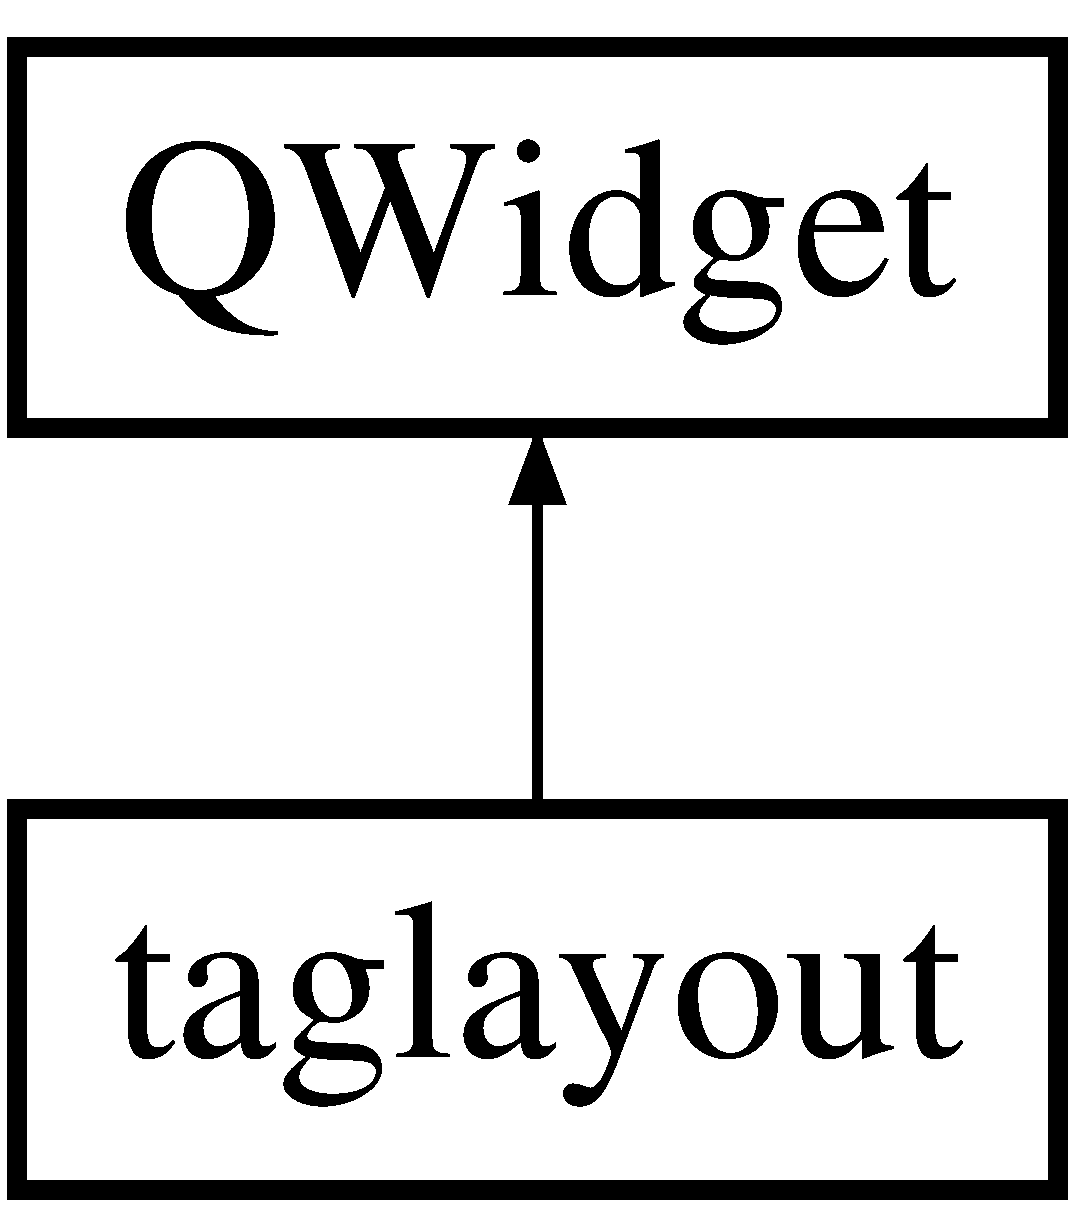
\includegraphics[height=2.000000cm]{classtaglayout}
\end{center}
\end{figure}
\subsection*{Public Slots}
\begin{DoxyCompactItemize}
\item 
\hypertarget{classtaglayout_ab885eac00ae5dabf14d05ad0466f8c40}{void \hyperlink{classtaglayout_ab885eac00ae5dabf14d05ad0466f8c40}{slot\-\_\-print\-\_\-\-Tags} ()}\label{classtaglayout_ab885eac00ae5dabf14d05ad0466f8c40}

\begin{DoxyCompactList}\small\item\em slot d'affichage des tags \end{DoxyCompactList}\item 
\hypertarget{classtaglayout_adc394329955e8887115f05a85377f940}{void \hyperlink{classtaglayout_adc394329955e8887115f05a85377f940}{slot\-\_\-del\-\_\-\-Tags} ()}\label{classtaglayout_adc394329955e8887115f05a85377f940}

\begin{DoxyCompactList}\small\item\em slot de suppression des tags \end{DoxyCompactList}\item 
\hypertarget{classtaglayout_ae21bbf293ba198e7876d7e5427d80852}{void \hyperlink{classtaglayout_ae21bbf293ba198e7876d7e5427d80852}{find\-Tag} ()}\label{classtaglayout_ae21bbf293ba198e7876d7e5427d80852}

\begin{DoxyCompactList}\small\item\em slot associé à la barre de recherche, permettant de chercher dans la liste des tags le tag souhaité \end{DoxyCompactList}\item 
\hypertarget{classtaglayout_ad1b120e1f0c5677577a579e648fe8a9e}{void \hyperlink{classtaglayout_ad1b120e1f0c5677577a579e648fe8a9e}{on\-\_\-tagbutton\-\_\-clicked} ()}\label{classtaglayout_ad1b120e1f0c5677577a579e648fe8a9e}

\begin{DoxyCompactList}\small\item\em slot associé au boutton de tag, permet soit l'affichage des tags associés soit de tagger un fichier \end{DoxyCompactList}\item 
\hypertarget{classtaglayout_a5bab3aa8a1c75f04e73bf0644e74cf1c}{void \hyperlink{classtaglayout_a5bab3aa8a1c75f04e73bf0644e74cf1c}{on\-\_\-filterbutton\-\_\-clicked} ()}\label{classtaglayout_a5bab3aa8a1c75f04e73bf0644e74cf1c}

\begin{DoxyCompactList}\small\item\em slot associé au boutton de tag pour le filtrage \end{DoxyCompactList}\end{DoxyCompactItemize}
\subsection*{Public Member Functions}
\begin{DoxyCompactItemize}
\item 
\hyperlink{classtaglayout_af32701e2f0dbfabc1b39a18dc2d65aad}{taglayout} (\hyperlink{classxmldom}{xmldom} $\ast$xd, \hyperlink{classexplorerlayout}{explorerlayout} $\ast$el)
\begin{DoxyCompactList}\small\item\em construteur de la classe \end{DoxyCompactList}\item 
\hypertarget{classtaglayout_af06d79cca2f358f06b47f335e95b1f63}{void \hyperlink{classtaglayout_af06d79cca2f358f06b47f335e95b1f63}{print\-\_\-\-Tags} ()}\label{classtaglayout_af06d79cca2f358f06b47f335e95b1f63}

\begin{DoxyCompactList}\small\item\em procedure affichant les tags dans la gridlayout \end{DoxyCompactList}\item 
Q\-Vector$<$ \hyperlink{classtag}{tag} $\ast$ $>$ $\ast$ \hyperlink{classtaglayout_a2e520044d1382d8327e1f952fc39558f}{get\-Tag\-List} ()
\begin{DoxyCompactList}\small\item\em fonction retournant la liste de tags \end{DoxyCompactList}\item 
Q\-Push\-Button $\ast$ \hyperlink{classtaglayout_a27c1f97e87c8ce6694b4069ef74183b6}{create\-Button} (\hyperlink{classtag}{tag} $\ast$\hyperlink{classtag}{tag})
\begin{DoxyCompactList}\small\item\em fonction permettant la création d'un boutton tag \end{DoxyCompactList}\item 
void \hyperlink{classtaglayout_a716e94f88343dc876375072f58e1b2d1}{add\-File} (Q\-String tagname, Q\-String file)
\begin{DoxyCompactList}\small\item\em procedure ajout un fichier a un tag \end{DoxyCompactList}\item 
\hyperlink{classaddtagdialog}{addtagdialog} $\ast$ \hyperlink{classtaglayout_a0e5bf2b22dd7cb27017d7e40020bf081}{get\-Dial} ()
\begin{DoxyCompactList}\small\item\em fonction créant la boite de dialog d'ajout \end{DoxyCompactList}\item 
\hyperlink{classdeltagdialog}{deltagdialog} $\ast$ \hyperlink{classtaglayout_a883465cdf9cedbde062f2ba60808a7fd}{get\-Del\-Dial} ()
\begin{DoxyCompactList}\small\item\em fonction créant la boite de dialog de suppression \end{DoxyCompactList}\end{DoxyCompactItemize}


\subsection{Constructor \& Destructor Documentation}
\hypertarget{classtaglayout_af32701e2f0dbfabc1b39a18dc2d65aad}{\index{taglayout@{taglayout}!taglayout@{taglayout}}
\index{taglayout@{taglayout}!taglayout@{taglayout}}
\subsubsection[{taglayout}]{\setlength{\rightskip}{0pt plus 5cm}taglayout\-::taglayout (
\begin{DoxyParamCaption}
\item[{{\bf xmldom} $\ast$}]{xd, }
\item[{{\bf explorerlayout} $\ast$}]{el}
\end{DoxyParamCaption}
)}}\label{classtaglayout_af32701e2f0dbfabc1b39a18dc2d65aad}


construteur de la classe 


\begin{DoxyParams}{Parameters}
{\em xd} & le xml genere à partir du fichier xml \\
\hline
{\em el} & explorer layout \\
\hline
\end{DoxyParams}


\subsection{Member Function Documentation}
\hypertarget{classtaglayout_a716e94f88343dc876375072f58e1b2d1}{\index{taglayout@{taglayout}!add\-File@{add\-File}}
\index{add\-File@{add\-File}!taglayout@{taglayout}}
\subsubsection[{add\-File}]{\setlength{\rightskip}{0pt plus 5cm}void taglayout\-::add\-File (
\begin{DoxyParamCaption}
\item[{Q\-String}]{tagname, }
\item[{Q\-String}]{file}
\end{DoxyParamCaption}
)}}\label{classtaglayout_a716e94f88343dc876375072f58e1b2d1}


procedure ajout un fichier a un tag 


\begin{DoxyParams}{Parameters}
{\em tagname} & le nom du tag \\
\hline
{\em file} & le nom du fichier \\
\hline
\end{DoxyParams}
\hypertarget{classtaglayout_a27c1f97e87c8ce6694b4069ef74183b6}{\index{taglayout@{taglayout}!create\-Button@{create\-Button}}
\index{create\-Button@{create\-Button}!taglayout@{taglayout}}
\subsubsection[{create\-Button}]{\setlength{\rightskip}{0pt plus 5cm}Q\-Push\-Button $\ast$ taglayout\-::create\-Button (
\begin{DoxyParamCaption}
\item[{{\bf tag} $\ast$}]{tag}
\end{DoxyParamCaption}
)}}\label{classtaglayout_a27c1f97e87c8ce6694b4069ef74183b6}


fonction permettant la création d'un boutton tag 


\begin{DoxyParams}{Parameters}
{\em tag} & \\
\hline
\end{DoxyParams}
\begin{DoxyReturn}{Returns}

\end{DoxyReturn}
\hypertarget{classtaglayout_a883465cdf9cedbde062f2ba60808a7fd}{\index{taglayout@{taglayout}!get\-Del\-Dial@{get\-Del\-Dial}}
\index{get\-Del\-Dial@{get\-Del\-Dial}!taglayout@{taglayout}}
\subsubsection[{get\-Del\-Dial}]{\setlength{\rightskip}{0pt plus 5cm}{\bf deltagdialog} $\ast$ taglayout\-::get\-Del\-Dial (
\begin{DoxyParamCaption}
{}
\end{DoxyParamCaption}
)}}\label{classtaglayout_a883465cdf9cedbde062f2ba60808a7fd}


fonction créant la boite de dialog de suppression 

\begin{DoxyReturn}{Returns}
l'adresse vers la boite 
\end{DoxyReturn}
\hypertarget{classtaglayout_a0e5bf2b22dd7cb27017d7e40020bf081}{\index{taglayout@{taglayout}!get\-Dial@{get\-Dial}}
\index{get\-Dial@{get\-Dial}!taglayout@{taglayout}}
\subsubsection[{get\-Dial}]{\setlength{\rightskip}{0pt plus 5cm}{\bf addtagdialog} $\ast$ taglayout\-::get\-Dial (
\begin{DoxyParamCaption}
{}
\end{DoxyParamCaption}
)}}\label{classtaglayout_a0e5bf2b22dd7cb27017d7e40020bf081}


fonction créant la boite de dialog d'ajout 

\begin{DoxyReturn}{Returns}
l'adresse vers la boite 
\end{DoxyReturn}
\hypertarget{classtaglayout_a2e520044d1382d8327e1f952fc39558f}{\index{taglayout@{taglayout}!get\-Tag\-List@{get\-Tag\-List}}
\index{get\-Tag\-List@{get\-Tag\-List}!taglayout@{taglayout}}
\subsubsection[{get\-Tag\-List}]{\setlength{\rightskip}{0pt plus 5cm}Q\-Vector$<$ {\bf tag} $\ast$ $>$ $\ast$ taglayout\-::get\-Tag\-List (
\begin{DoxyParamCaption}
{}
\end{DoxyParamCaption}
)}}\label{classtaglayout_a2e520044d1382d8327e1f952fc39558f}


fonction retournant la liste de tags 

\begin{DoxyReturn}{Returns}
Q\-Vector de tag 
\end{DoxyReturn}


The documentation for this class was generated from the following files\-:\begin{DoxyCompactItemize}
\item 
\hyperlink{taglayout_8hpp}{taglayout.\-hpp}\item 
taglayout.\-cpp\end{DoxyCompactItemize}

\hypertarget{classxmldom}{\section{xmldom Class Reference}
\label{classxmldom}\index{xmldom@{xmldom}}
}
Inheritance diagram for xmldom\-:\begin{figure}[H]
\begin{center}
\leavevmode
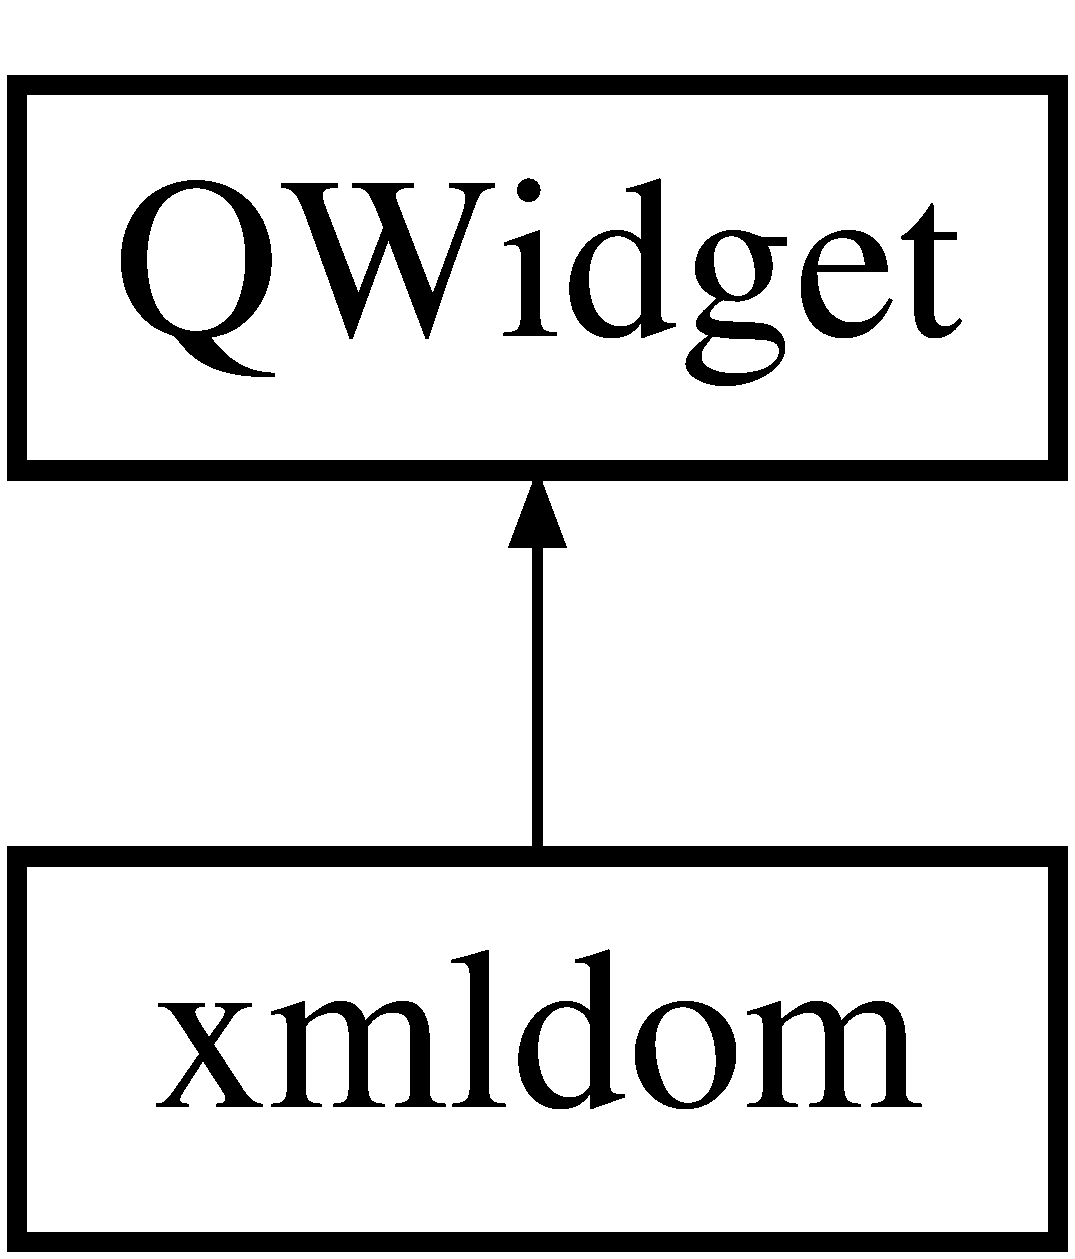
\includegraphics[height=2.000000cm]{classxmldom}
\end{center}
\end{figure}
\subsection*{Public Slots}
\begin{DoxyCompactItemize}
\item 
\hypertarget{classxmldom_a4eaf8365402c252d1056b031c06bc94f}{void \hyperlink{classxmldom_a4eaf8365402c252d1056b031c06bc94f}{xml\-Saver} ()}\label{classxmldom_a4eaf8365402c252d1056b031c06bc94f}

\begin{DoxyCompactList}\small\item\em slot permettant l'enregistrement dans le fichier xml \end{DoxyCompactList}\end{DoxyCompactItemize}
\subsection*{Public Member Functions}
\begin{DoxyCompactItemize}
\item 
\hypertarget{classxmldom_ad072d12232c0cd4b25d3c5241baf4cf0}{\hyperlink{classxmldom_ad072d12232c0cd4b25d3c5241baf4cf0}{xmldom} ()}\label{classxmldom_ad072d12232c0cd4b25d3c5241baf4cf0}

\begin{DoxyCompactList}\small\item\em constructeur par defaut de la classe. \end{DoxyCompactList}\item 
\hyperlink{classxmldom_acb5340a747b9623a2d9294bbbfa39774}{xmldom} (Q\-String filepath)
\begin{DoxyCompactList}\small\item\em constructeur de la classe prenant le chemin du fichier \end{DoxyCompactList}\item 
\hypertarget{classxmldom_af4a0f240c83121ac2cbb75b181cb095f}{\hyperlink{classxmldom_af4a0f240c83121ac2cbb75b181cb095f}{$\sim$xmldom} ()}\label{classxmldom_af4a0f240c83121ac2cbb75b181cb095f}

\begin{DoxyCompactList}\small\item\em destructeur de la classe \end{DoxyCompactList}\item 
\hypertarget{classxmldom_a1b066769999c193a6565b1dfaa6b2f30}{void \hyperlink{classxmldom_a1b066769999c193a6565b1dfaa6b2f30}{xml\-Open} ()}\label{classxmldom_a1b066769999c193a6565b1dfaa6b2f30}

\begin{DoxyCompactList}\small\item\em procedure ouvrant un fichier xml \end{DoxyCompactList}\item 
\hypertarget{classxmldom_afee9a603705a4fbe1763d0e2d2b59e3e}{void \hyperlink{classxmldom_afee9a603705a4fbe1763d0e2d2b59e3e}{xml\-Reader} ()}\label{classxmldom_afee9a603705a4fbe1763d0e2d2b59e3e}

\begin{DoxyCompactList}\small\item\em procedure lisant un fichier xml \end{DoxyCompactList}\item 
void \hyperlink{classxmldom_ac88d355800d4899937d77cd90b1a5cdb}{add\-Tag} (Q\-String s, Q\-Color c)
\begin{DoxyCompactList}\small\item\em procedure créant un tag à partir des balises xml \end{DoxyCompactList}\item 
Q\-Vector$<$ \hyperlink{classtag}{tag} $\ast$ $>$ $\ast$ \hyperlink{classxmldom_a5e98ced4b5518ee5cea38a33bc05922f}{get\-Tag\-List} ()
\begin{DoxyCompactList}\small\item\em fonction retournant l'adresse du tableau de tags \end{DoxyCompactList}\item 
\hypertarget{classxmldom_a16088fab1089a12869b7d70faf3118e7}{void \hyperlink{classxmldom_a16088fab1089a12869b7d70faf3118e7}{save\-Tag\-List\-To\-X\-M\-L} ()}\label{classxmldom_a16088fab1089a12869b7d70faf3118e7}

\begin{DoxyCompactList}\small\item\em procedure transformant une tagliste en xml \end{DoxyCompactList}\item 
void \hyperlink{classxmldom_aefd0dc1ccf2d1ea6d5d523dba0b51113}{add\-File} (Q\-Dom\-Element root, Q\-String path)
\begin{DoxyCompactList}\small\item\em procedure ajoutant une balise file \end{DoxyCompactList}\end{DoxyCompactItemize}


\subsection{Constructor \& Destructor Documentation}
\hypertarget{classxmldom_acb5340a747b9623a2d9294bbbfa39774}{\index{xmldom@{xmldom}!xmldom@{xmldom}}
\index{xmldom@{xmldom}!xmldom@{xmldom}}
\subsubsection[{xmldom}]{\setlength{\rightskip}{0pt plus 5cm}xmldom\-::xmldom (
\begin{DoxyParamCaption}
\item[{Q\-String}]{filepath}
\end{DoxyParamCaption}
)}}\label{classxmldom_acb5340a747b9623a2d9294bbbfa39774}


constructeur de la classe prenant le chemin du fichier 


\begin{DoxyParams}{Parameters}
{\em filepath} & chemin du fichier xml \\
\hline
\end{DoxyParams}


\subsection{Member Function Documentation}
\hypertarget{classxmldom_aefd0dc1ccf2d1ea6d5d523dba0b51113}{\index{xmldom@{xmldom}!add\-File@{add\-File}}
\index{add\-File@{add\-File}!xmldom@{xmldom}}
\subsubsection[{add\-File}]{\setlength{\rightskip}{0pt plus 5cm}void xmldom\-::add\-File (
\begin{DoxyParamCaption}
\item[{Q\-Dom\-Element}]{root, }
\item[{Q\-String}]{path}
\end{DoxyParamCaption}
)}}\label{classxmldom_aefd0dc1ccf2d1ea6d5d523dba0b51113}


procedure ajoutant une balise file 


\begin{DoxyParams}{Parameters}
{\em root} & noeud parent du fichier \\
\hline
{\em path} & chemin du fichiers \\
\hline
\end{DoxyParams}
\hypertarget{classxmldom_ac88d355800d4899937d77cd90b1a5cdb}{\index{xmldom@{xmldom}!add\-Tag@{add\-Tag}}
\index{add\-Tag@{add\-Tag}!xmldom@{xmldom}}
\subsubsection[{add\-Tag}]{\setlength{\rightskip}{0pt plus 5cm}void xmldom\-::add\-Tag (
\begin{DoxyParamCaption}
\item[{Q\-String}]{s, }
\item[{Q\-Color}]{c}
\end{DoxyParamCaption}
)}}\label{classxmldom_ac88d355800d4899937d77cd90b1a5cdb}


procedure créant un tag à partir des balises xml 


\begin{DoxyParams}{Parameters}
{\em s} & nom du tag \\
\hline
{\em c} & couleur du tag \\
\hline
\end{DoxyParams}
\hypertarget{classxmldom_a5e98ced4b5518ee5cea38a33bc05922f}{\index{xmldom@{xmldom}!get\-Tag\-List@{get\-Tag\-List}}
\index{get\-Tag\-List@{get\-Tag\-List}!xmldom@{xmldom}}
\subsubsection[{get\-Tag\-List}]{\setlength{\rightskip}{0pt plus 5cm}Q\-Vector$<$ {\bf tag} $\ast$ $>$ $\ast$ xmldom\-::get\-Tag\-List (
\begin{DoxyParamCaption}
{}
\end{DoxyParamCaption}
)}}\label{classxmldom_a5e98ced4b5518ee5cea38a33bc05922f}


fonction retournant l'adresse du tableau de tags 

\begin{DoxyReturn}{Returns}
l'adresse du tableau de tag 
\end{DoxyReturn}


The documentation for this class was generated from the following files\-:\begin{DoxyCompactItemize}
\item 
\hyperlink{xmldom_8hpp}{xmldom.\-hpp}\item 
xmldom.\-cpp\end{DoxyCompactItemize}

\chapter{File Documentation}
\hypertarget{addtagdialog_8hpp}{\section{addtagdialog.\-hpp File Reference}
\label{addtagdialog_8hpp}\index{addtagdialog.\-hpp@{addtagdialog.\-hpp}}
}


classe permettant l'affichage de la boite de dialog d'ajout d'un tag  


{\ttfamily \#include \char`\"{}tag.\-hpp\char`\"{}}\\*
{\ttfamily \#include \char`\"{}xmldom.\-hpp\char`\"{}}\\*
{\ttfamily \#include $<$Q\-Dialog$>$}\\*
{\ttfamily \#include $<$Q\-Line\-Edit$>$}\\*
{\ttfamily \#include $<$Q\-H\-Box\-Layout$>$}\\*
{\ttfamily \#include $<$Q\-Message\-Box$>$}\\*
{\ttfamily \#include $<$Q\-Color$>$}\\*
{\ttfamily \#include $<$Q\-Push\-Button$>$}\\*
{\ttfamily \#include $<$Q\-Pixmap$>$}\\*
{\ttfamily \#include $<$Q\-Painter$>$}\\*
{\ttfamily \#include $<$Q\-Debug$>$}\\*
{\ttfamily \#include $<$Q\-Rgb$>$}\\*
{\ttfamily \#include $<$Q\-List$>$}\\*
{\ttfamily \#include $<$Q\-List\-Widget$>$}\\*
{\ttfamily \#include $<$Q\-Combo\-Box$>$}\\*
{\ttfamily \#include $<$Q\-Map$>$}\\*
\subsection*{Classes}
\begin{DoxyCompactItemize}
\item 
class \hyperlink{classaddtagdialog}{addtagdialog}
\end{DoxyCompactItemize}


\subsection{Detailed Description}
classe permettant l'affichage de la boite de dialog d'ajout d'un tag \begin{DoxyAuthor}{Authors}
Espasa Kévin, Bonnaud Jonathan 
\end{DoxyAuthor}

\hypertarget{deltagdialog_8hpp}{\section{deltagdialog.\-hpp File Reference}
\label{deltagdialog_8hpp}\index{deltagdialog.\-hpp@{deltagdialog.\-hpp}}
}


classe permettant l'affichage de la boite de dialog de suppression d'un ou plusieurs tags  


{\ttfamily \#include \char`\"{}tag.\-hpp\char`\"{}}\\*
{\ttfamily \#include \char`\"{}xmldom.\-hpp\char`\"{}}\\*
{\ttfamily \#include $<$Q\-Dialog$>$}\\*
{\ttfamily \#include $<$Q\-Line\-Edit$>$}\\*
{\ttfamily \#include $<$Q\-H\-Box\-Layout$>$}\\*
{\ttfamily \#include $<$Q\-Message\-Box$>$}\\*
{\ttfamily \#include $<$Q\-Color$>$}\\*
{\ttfamily \#include $<$Q\-Push\-Button$>$}\\*
{\ttfamily \#include $<$Q\-Debug$>$}\\*
{\ttfamily \#include $<$Q\-List$>$}\\*
{\ttfamily \#include $<$Q\-List\-Widget$>$}\\*
\subsection*{Classes}
\begin{DoxyCompactItemize}
\item 
class \hyperlink{classdeltagdialog}{deltagdialog}
\end{DoxyCompactItemize}


\subsection{Detailed Description}
classe permettant l'affichage de la boite de dialog de suppression d'un ou plusieurs tags \begin{DoxyAuthor}{Authors}
Espasa Kévin, Bonnaud Jonathan 
\end{DoxyAuthor}

\hypertarget{explorerlayout_8hpp}{\section{explorerlayout.\-hpp File Reference}
\label{explorerlayout_8hpp}\index{explorerlayout.\-hpp@{explorerlayout.\-hpp}}
}


widget affichant les fichiers et les informations qui sont associées  


{\ttfamily \#include \char`\"{}xmldom.\-hpp\char`\"{}}\\*
{\ttfamily \#include $<$Q\-Widget$>$}\\*
{\ttfamily \#include $<$Q\-Object$>$}\\*
{\ttfamily \#include $<$Q\-File\-System\-Model$>$}\\*
{\ttfamily \#include $<$Q\-Table\-View$>$}\\*
{\ttfamily \#include $<$Q\-V\-Box\-Layout$>$}\\*
{\ttfamily \#include $<$Q\-Line\-Edit$>$}\\*
{\ttfamily \#include $<$Q\-String$>$}\\*
{\ttfamily \#include $<$Q\-Dir$>$}\\*
{\ttfamily \#include $<$Q\-Message\-Box$>$}\\*
{\ttfamily \#include $<$Q\-Push\-Button$>$}\\*
{\ttfamily \#include $<$iostream$>$}\\*
{\ttfamily \#include $<$Q\-Header\-View$>$}\\*
{\ttfamily \#include $<$Q\-Completer$>$}\\*
{\ttfamily \#include $<$Q\-Dir\-Model$>$}\\*
{\ttfamily \#include $<$Q\-List\-Widget$>$}\\*
{\ttfamily \#include $<$Q\-Item\-Selection\-Model$>$}\\*
{\ttfamily \#include $<$Q\-Debug$>$}\\*
\subsection*{Classes}
\begin{DoxyCompactItemize}
\item 
class \hyperlink{classexplorerlayout}{explorerlayout}
\end{DoxyCompactItemize}


\subsection{Detailed Description}
widget affichant les fichiers et les informations qui sont associées \begin{DoxyAuthor}{Authors}
Espasa Kévin, Bonnaud Jonathan 
\end{DoxyAuthor}

\hypertarget{tag_8hpp}{\section{tag.\-hpp File Reference}
\label{tag_8hpp}\index{tag.\-hpp@{tag.\-hpp}}
}


classe definissant un tag  


{\ttfamily \#include $<$Q\-Color$>$}\\*
{\ttfamily \#include $<$Q\-Vector$>$}\\*
{\ttfamily \#include $<$Q\-String$>$}\\*
{\ttfamily \#include $<$Q\-File$>$}\\*
\subsection*{Classes}
\begin{DoxyCompactItemize}
\item 
class \hyperlink{classtag}{tag}
\end{DoxyCompactItemize}


\subsection{Detailed Description}
classe definissant un tag \begin{DoxyAuthor}{Authors}
Espasa Kévin, Bonnaud Jonathan 
\end{DoxyAuthor}

\hypertarget{taglayout_8hpp}{\section{taglayout.\-hpp File Reference}
\label{taglayout_8hpp}\index{taglayout.\-hpp@{taglayout.\-hpp}}
}


classe definissant les tags  


{\ttfamily \#include \char`\"{}tag.\-hpp\char`\"{}}\\*
{\ttfamily \#include \char`\"{}xmldom.\-hpp\char`\"{}}\\*
{\ttfamily \#include \char`\"{}addtagdialog.\-hpp\char`\"{}}\\*
{\ttfamily \#include \char`\"{}deltagdialog.\-hpp\char`\"{}}\\*
{\ttfamily \#include \char`\"{}explorerlayout.\-hpp\char`\"{}}\\*
{\ttfamily \#include $<$Q\-Line\-Edit$>$}\\*
{\ttfamily \#include $<$Q\-Label$>$}\\*
{\ttfamily \#include $<$Q\-Push\-Button$>$}\\*
{\ttfamily \#include $<$Q\-V\-Box\-Layout$>$}\\*
{\ttfamily \#include $<$Q\-Message\-Box$>$}\\*
{\ttfamily \#include $<$Q\-Object$>$}\\*
{\ttfamily \#include $<$Q\-Application$>$}\\*
{\ttfamily \#include $<$Q\-List\-Widget$>$}\\*
{\ttfamily \#include $<$Q\-Tab\-Bar$>$}\\*
\subsection*{Classes}
\begin{DoxyCompactItemize}
\item 
class \hyperlink{classtaglayout}{taglayout}
\end{DoxyCompactItemize}


\subsection{Detailed Description}
classe definissant les tags \begin{DoxyAuthor}{Authors}
Espasa Kévin, Bonnaud Jonathan 
\end{DoxyAuthor}

\hypertarget{xmldom_8hpp}{\section{xmldom.\-hpp File Reference}
\label{xmldom_8hpp}\index{xmldom.\-hpp@{xmldom.\-hpp}}
}


classe permettant la lecture et l'ecrire d'un xml  


{\ttfamily \#include \char`\"{}tag.\-hpp\char`\"{}}\\*
{\ttfamily \#include $<$Qt\-Xml/qxml.\-h$>$}\\*
{\ttfamily \#include $<$Q\-Dom\-Document$>$}\\*
{\ttfamily \#include $<$Q\-String$>$}\\*
{\ttfamily \#include $<$Q\-Widget$>$}\\*
{\ttfamily \#include $<$Q\-Dir$>$}\\*
{\ttfamily \#include $<$Q\-Message\-Box$>$}\\*
{\ttfamily \#include $<$iostream$>$}\\*
{\ttfamily \#include $<$Q\-Debug$>$}\\*
\subsection*{Classes}
\begin{DoxyCompactItemize}
\item 
class \hyperlink{classxmldom}{xmldom}
\end{DoxyCompactItemize}


\subsection{Detailed Description}
classe permettant la lecture et l'ecrire d'un xml \begin{DoxyAuthor}{Authors}
Espasa Kévin, Bonnaud Jonathan 
\end{DoxyAuthor}

%--- End generated contents ---

% Index
\newpage
\phantomsection
\addcontentsline{toc}{chapter}{Index}
\printindex

\end{document}
